
\setlength\fboxrule{0pt}
\begin{center}
	\fcolorbox{white}{white!100}{
		\fbox{



	\begin{minipage}{13em}
	\begin{center}      	
		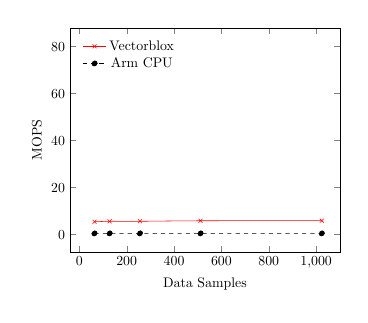
\begin{tikzpicture}[scale=0.5]
		\begin{axis}[
		xlabel=Data Samples,
		enlarge y limits = true,
		ylabel=MOPS,
		ymax = 80,
		xmax = 1100,
		legend pos=north west,
		legend style={draw=none}
		]
		%vbx
		\addplot [smooth,mark=x,red] plot coordinates {
			(64,     5.451)
			(128,    5.661)
			(256,    5.661)
			(512,    5.888)
			(1024,   5.924)			
		};
		%arm
		\addplot [smooth,mark=*,dashed] plot coordinates {
			(64,     0.497)
			(128,    0.506)
			(256,    0.507)
			(512,    0.508)
			(1024,   0.509)
			
		};
		\legend{Vectorblox\\Arm CPU\\}
		\end{axis}
		\end{tikzpicture}
	\end{center}  
	\tiny  
	Vectorblox C API Implementation in Comparison with naive C Implementation on ARM CPU.
	\end{minipage}

	\hspace{1em}
	\begin{minipage}{13em}
	\begin{center}      				
	 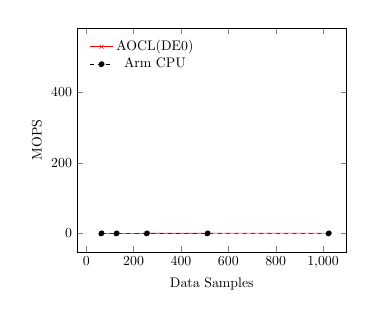
\begin{tikzpicture}[scale=0.5]
	 \begin{axis}[
	 xlabel=Data Samples,
	 ylabel=MOPS,
	 enlarge y limits = true,
	 ymax = 530,
	 xmax = 1100,
	 legend pos=north west,
	 legend style={draw=none}
	 ]
	 \addplot [smooth,mark=x,red] plot coordinates {
			(64,     0.1301)
			(128,    0.2378)
			(256,    0.4532)
			(512,    0.5793)
			(1024,   1.0483)			
		};
		\addplot [smooth,mark=*,dashed] plot coordinates {
			(64,     0.00570)
			(128,    0.01089)
			(256,    0.0208)
			(512,    0.0383)
			(1024,   0.0710)
			
		};
	 \legend{AOCL(DE0)\\Arm CPU\\}
	 \end{axis}
	 \end{tikzpicture}
	\end{center}
	\tiny 
	OpenCL Implementation Timing Comparison between ARM CPU and AOCL FPGA Implementation.   					
	\end{minipage}
					
		}
	}
\end{center}


